\section{Introduction}

% % General params
\newcommand{\mainLineWidth}{1}
\newcommand{\embedLineWidth}{2}
\newcommand{\bigDeltaY}{1}
\newcommand{\smallDeltaY}{0.5}
\newcommand{\offsetY}{0.5}


% objrel
\newcommand{\objrelX}{0}
\newcommand{\objrelY}{0}
\newcommand{\objrelMainSubjectX}{-3}
\newcommand{\objrelMainVerbX}{2}
\newcommand{\objrelEmbedSubjectX}{-0.5}
\newcommand{\objrelEmbedVerbX}{0.9}

% mental-SR
\newcommand{\mentalSRX}{0}
\newcommand{\mentalSRY}{-3}
\newcommand{\mentalSRMainSubjectX}{-2.7}
\newcommand{\mentalSRMainVerbX}{-1.6}
\newcommand{\mentalSREmbedSubjectX}{0.5}
\newcommand{\mentalSREmbedVerbX}{1.8}

% objrel-nounpp
\newcommand{\objrelNounppX}{0}
\newcommand{\objrelNounppY}{-6}
\newcommand{\objrelNounppMainSubjectX}{-4}
\newcommand{\objrelNounppMainVerbX}{3.5}
\newcommand{\objrelNounppEmbedSubjectX}{-1.8}
\newcommand{\objrelNounppEmbedVerbX}{2.2}

% mental-LR
\newcommand{\mentalLRX}{0}
\newcommand{\mentalLRY}{-9}
\newcommand{\mentalLRMainSubjectX}{-4}
\newcommand{\mentalLRMainVerbX}{-2.8}
\newcommand{\mentalLREmbedSubjectX}{-0.8}
\newcommand{\mentalLREmbedVerbX}{3.2}


\begin{figure*}
\centering
\makebox[5cm][c]{%
\begin{minipage}{.9\textwidth}
    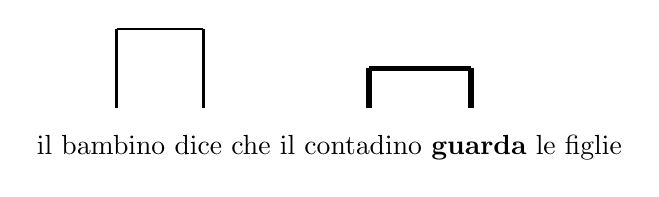
\begin{tikzpicture}
        % Sentence
        \node[align=left] at (\mentalSRX,\mentalSRY) {il bambino dice che il contadino \textbf{guarda} le figlie};
        
        % Draw main dependency
        \draw [line width=\mainLineWidth, black] (\mentalSRX+\mentalSRMainSubjectX,\mentalSRY+\offsetY) -- (\mentalSRX+\mentalSRMainSubjectX,\mentalSRY+\offsetY+\bigDeltaY);
        \draw [line width=\mainLineWidth, black] (\mentalSRX+\mentalSRMainSubjectX,\mentalSRY+\offsetY+\bigDeltaY) -- (\mentalSRX+\mentalSRMainVerbX,\mentalSRY+\offsetY+\bigDeltaY);
        \draw [line width=\mainLineWidth, black] (\mentalSRX+\mentalSRMainVerbX,\mentalSRY+\offsetY+\bigDeltaY) -- (\mentalSRX+\mentalSRMainVerbX,\mentalSRY+\offsetY);
    
        % Draw embedded dependency
        \draw [line width=\embedLineWidth, black] (\mentalSRX+\mentalSREmbedSubjectX,\mentalSRY+\offsetY) -- (\mentalSRX+\mentalSREmbedSubjectX,\mentalSRY+\offsetY+\smallDeltaY);
        \draw [line width=\embedLineWidth, black] (\mentalSRX+\mentalSREmbedSubjectX,\mentalSRY+\offsetY+\smallDeltaY) -- (\mentalSRX+\mentalSREmbedVerbX,\mentalSRY+\offsetY+\smallDeltaY);
        \draw [line width=\embedLineWidth, black] (\mentalSRX+\mentalSREmbedVerbX,\mentalSRY+\offsetY+\smallDeltaY) -- (\mentalSRX+\mentalSREmbedVerbX,\mentalSRY+\offsetY);
    \end{tikzpicture}
\end{minipage}
}


\makebox[5cm][c]{%
\begin{minipage}{.9\textwidth}
    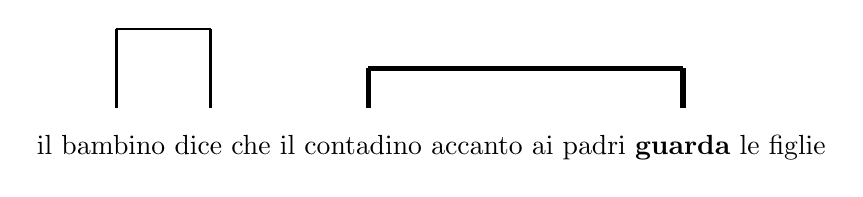
\begin{tikzpicture}
        % Sentence
        \node[align=left] at (\mentalLRX,\mentalLRY) {il bambino dice che il contadino accanto ai padri \textbf{guarda} le figlie};
        
        % Draw main dependency
        \draw [line width=\mainLineWidth, black] (\mentalLRX+\mentalLRMainSubjectX,\mentalLRY+\offsetY) -- (\mentalLRX+\mentalLRMainSubjectX,\mentalLRY+\offsetY+\bigDeltaY);
        \draw [line width=\mainLineWidth, black] (\mentalLRX+\mentalLRMainSubjectX,\mentalLRY+\offsetY+\bigDeltaY) -- (\mentalLRX+\mentalLRMainVerbX,\mentalLRY+\offsetY+\bigDeltaY);
        \draw [line width=\mainLineWidth, black] (\mentalLRX+\mentalLRMainVerbX,\mentalLRY+\offsetY+\bigDeltaY) -- (\mentalLRX+\mentalLRMainVerbX,\mentalLRY+\offsetY);
    
        % Draw embedded dependency
        \draw [line width=\embedLineWidth, black] (\mentalLRX+\mentalLREmbedSubjectX,\mentalLRY+\offsetY) -- (\mentalLRX+\mentalLREmbedSubjectX,\mentalLRY+\offsetY+\smallDeltaY);
        \draw [line width=\embedLineWidth, black] (\mentalLRX+\mentalLREmbedSubjectX,\mentalLRY+\offsetY+\smallDeltaY) -- (\mentalLRX+\mentalLREmbedVerbX,\mentalLRY+\offsetY+\smallDeltaY);
        \draw [line width=\embedLineWidth, black] (\mentalLRX+\mentalLREmbedVerbX,\mentalLRY+\offsetY+\smallDeltaY) -- (\mentalLRX+\mentalLREmbedVerbX,\mentalLRY+\offsetY);
    \end{tikzpicture}
\end{minipage}
}%


\makebox[5cm][c]{%
\begin{minipage}{.9\textwidth}
     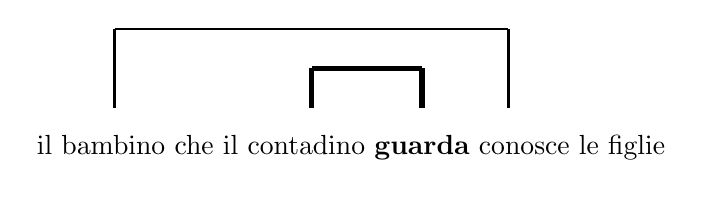
\begin{tikzpicture}
        % Sentence
        \node[align=left] at (\objrelX,\objrelY) {il bambino che il contadino \textbf{guarda} conosce le figlie};
        
        % Draw main dependency
        \draw [line width=\mainLineWidth, black] (\objrelX+\objrelMainSubjectX,\objrelY+\offsetY) -- (\objrelX+\objrelMainSubjectX,\objrelY+\offsetY+\bigDeltaY);
        \draw [line width=\mainLineWidth, black] (\objrelX+\objrelMainSubjectX,\objrelY+\offsetY+\bigDeltaY) -- (\objrelX+\objrelMainVerbX,\objrelY+\offsetY+\bigDeltaY);
        \draw [line width=\mainLineWidth, black] (\objrelX+\objrelMainVerbX,\objrelY+\offsetY+\bigDeltaY) -- (\objrelX+\objrelMainVerbX,\objrelY+\offsetY);
    
        % Draw embedded dependency
        \draw [line width=\embedLineWidth, black] (\objrelX+\objrelEmbedSubjectX,\objrelY+\offsetY) -- (\objrelX+\objrelEmbedSubjectX,\objrelY+\offsetY+\smallDeltaY);
        \draw [line width=\embedLineWidth, black] (\objrelX+\objrelEmbedSubjectX,\objrelY+\offsetY+\smallDeltaY) -- (\objrelX+\objrelEmbedVerbX,\objrelY+\offsetY+\smallDeltaY);
        \draw [line width=\embedLineWidth, black] (\objrelX+\objrelEmbedVerbX,\objrelY+\offsetY+\smallDeltaY) -- (\objrelX+\objrelEmbedVerbX,\objrelY+\offsetY);
    \end{tikzpicture}
\end{minipage}
}%


\makebox[5cm][c]{%
\begin{minipage}{.9\textwidth}
    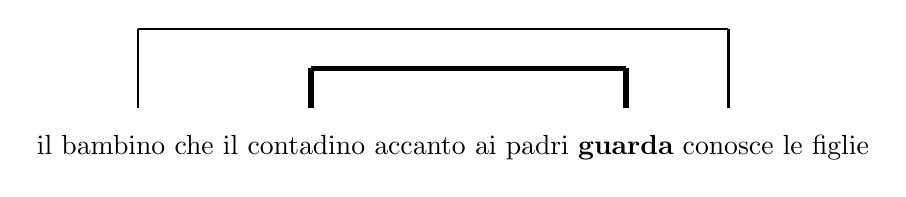
\begin{tikzpicture}
        % Sentence
        \node[align=left] at (\objrelNounppX,\objrelNounppY) {il bambino che il contadino accanto ai padri \textbf{guarda} conosce le figlie};
        
        % Draw main dependency
        \draw [line width=\mainLineWidth, black] (\objrelNounppX+\objrelNounppMainSubjectX,\objrelNounppY+\offsetY) -- (\objrelNounppX+\objrelNounppMainSubjectX,\objrelNounppY+\offsetY+\bigDeltaY);
        \draw [line width=\mainLineWidth, black] (\objrelNounppX+\objrelNounppMainSubjectX,\objrelNounppY+\offsetY+\bigDeltaY) -- (\objrelNounppX+\objrelNounppMainVerbX,\objrelNounppY+\offsetY+\bigDeltaY);
        \draw [line width=\mainLineWidth, black] (\objrelNounppX+\objrelNounppMainVerbX,\objrelNounppY+\offsetY+\bigDeltaY) -- (\objrelNounppX+\objrelNounppMainVerbX,\objrelNounppY+\offsetY);
    
        % Draw embedded dependency
        \draw [line width=\embedLineWidth, black] (\objrelNounppX+\objrelNounppEmbedSubjectX,\objrelNounppY+\offsetY) -- (\objrelNounppX+\objrelNounppEmbedSubjectX,\objrelNounppY+\offsetY+\smallDeltaY);
        \draw [line width=\embedLineWidth, black] (\objrelNounppX+\objrelNounppEmbedSubjectX,\objrelNounppY+\offsetY+\smallDeltaY) -- (\objrelNounppX+\objrelNounppEmbedVerbX,\objrelNounppY+\offsetY+\smallDeltaY);
        \draw [line width=\embedLineWidth, black] (\objrelNounppX+\objrelNounppEmbedVerbX,\objrelNounppY+\offsetY+\smallDeltaY) -- (\objrelNounppX+\objrelNounppEmbedVerbX,\objrelNounppY+\offsetY);
    \end{tikzpicture}
\end{minipage}
}%
    %         \end{tikzpicture}
    \caption{Design} 
\end{figure*}
    

\begin{itemize}
\item Neural language models (NLMs) are wonderful blah blah blah, revived interest in
  looking at them as computational models of language processing
\item Current research in the area focuses on understanding the behaviour of NLMs wrt
  various grammatical phenomena; some work showing correlations
  between internal states and said phenomena
\item Number agreement is an area where some steps have been taken
  towards mechanistic understanding:
  \begin{itemize}
  \item sparse feature-propagation mechanism controlled by distributed
    grammar network
  \end{itemize}
\item Our goal here is two-fold:
  \begin{itemize}
  \item First, we replicate our earlier results on the emergence of
    this mechanism in a different language, as well as extending them to a different
    agreement phenomenon (\textbf{do we?}) confirming it is no fluke
  \item Second, we use our understanding of of how agreement is
    performed by NLMs to make a new prediction about a difficulty in agreement
    processing in humans (analogy to DiCarlo's work in vision?)
  \end{itemize}
\item Main result: the predicted pattern is confirmed; however, in other ways,
  human and NLM patterns differ, confirming that studying NLMs is
  productive, but the right perspective is not to treat them as
  full-fledged cognitive models, but rather as powerful computational
  systems that, when faced with challenges similar to those
  encountered by humans, might adopt partially analogous solutions
\end{itemize}
